\documentclass{report}

\usepackage{graphicx} % Required for inserting images
\usepackage{float}
\usepackage{amsmath}
\usepackage{color}
\usepackage{url}
\usepackage{hyperref}
\usepackage{geometry}
%\usepackage[margin=10mm]{geometry}
\setlength{\evensidemargin}{10mm}
\setlength{\oddsidemargin}{5mm}


\title{Software courses}
\author{Daniele Schlagenauf}
\date{June 2024}

\begin{document}

\maketitle

\chapter{Git}

\paragraph{Exam notes}
The exam is formed by:
\begin{itemize}
    \item Homework: Create an account with a repository on GitHub and perform first git push
    \item Multiple choice question, 30 question in google format  
\end{itemize}
In all the cases, notes book etc are allowed.

\paragraph{Version Control System}
Known as VCS are system develop to \textbf{store the changes} of a file over time, eventually recall them. Can be different type
\begin{itemize}
    \item \textit{Local}: Not share info, everything stay on the same machine 
    \item \textit{Centralized}:  A single copy, which everybody download and then modify before 
    update
    \item \textit{Distributed}: Each user has own copy then all sync together 
\end{itemize}

\section{Git}
Git is one of the most famous VCS, do not work well with too large file, binary file (or pdf) and with sensitive data since shared. While is largely since fasst, secure, open source and scalable.
\vspace{2mm}
Git can be use both \textbf{CLI} (Command Line Interface) or \textbf{GUI} (Graphical User Interface), the first allow a most powerful but complex approach while the second is more understandable by humans beings but limited option and not flexible as CLI.

The main structure is: 
\begin{figure}[H]
    \centering
    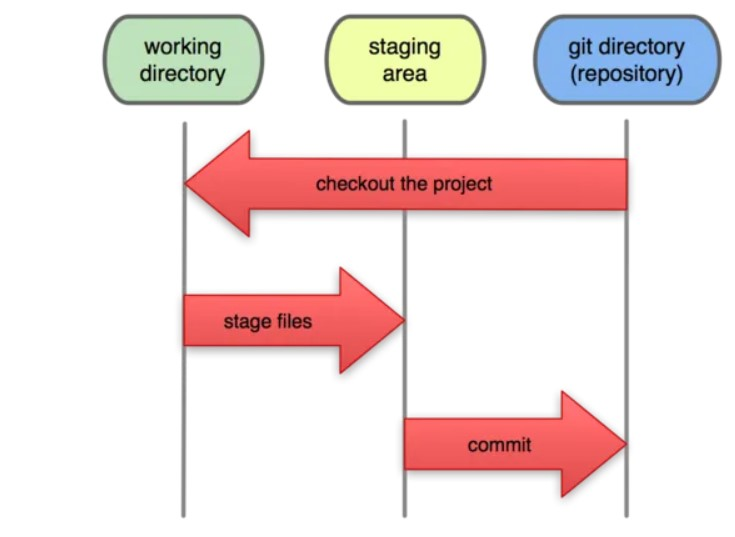
\includegraphics[scale=0.5]{img/git1.jpg}
    \caption{Structure of git}
    \label{git_str}
\end{figure}
Where the \textit{working directory} is the local folder where the file are stored and modified, the \textit{staging area} is a middle step to compute before the commit abd stay on the local machine while with a commit is possible to store the new files on the \textit{Git repository}

\subsection{Command}
The main CLI command will be show, in particular the blue ones will refer to the used of branches, for a intermediate approach while in red the more advanced ones:
\begin{itemize}
    \item \textbf{git init}: start the filder to git 
    \item \textbf{git add}: Command need to pass from working dir to staging area, after a space is possible to add the $<filename>$ to add, with extension, or with the . add all the changes.
    \item \textbf{git commit -m "msg"}: create a commit with the comment on what is change inside
    \item \textbf{git push}: commit the file on Github (after setting show in \autoref{GitHub})
    \item  \textbf{git mv $<old.txt> <newfile.txt>$}: allow renomination of file without lose the track of the changes
    \item \textbf{git reset}: Allow to recover an add file (reverse of add!)
    \item  \textbf{git diff}: compute the difference between working and stage area, should need a proper IDE to be human understandable. (--staged: diff between stage and commit)
    \item \textbf{git log}: Allow to visualize the list of commit done on the repository. Some option are --graph (color, use mainly for branches), --oneline (shorter versione) --$<name>$ (see the log of specific file) 
    \item \textcolor{blue}{git checkout -b \textless branchName \textgreater}: Create a new branch with the given name if not already created
     \item \textcolor{blue}{git log --graph --all}: now the branch is more visible 
     \item \textcolor{blue}{git push origin feature}: commit only the branch not the main
     \item \textcolor{blue}{git switch \textless branchName \textgreater}: allow to switch from the branch to the one specified
     \item \textcolor{blue}{git merge \textless branchName \textgreater}: from the directory of the branch that should be receive the merge (main mainly), specify which branch merge \newline
     \textbf{Possible conflict}: some conflict could happen when try to merge a file that is modified in both branches. The idea is work on files only in the external branch not touch the one on the internal ones and allow a single person/group on each file hence known what was modified.
     \item \textcolor{red}{git config --global alias}: create a routine, that can be run instead of a very large command
    \item \textcolor{red}{git commit --amend}: delete the last commit, use when forget a file, or commit something wrong. If add \textbf{-m "new\_msg} change only the commit message, for example for type error
    \item \textcolor{red}{git revert \textless commit \textgreater}: delete the commit specify and commit the actual one 
    \item \textcolor{red}{git reflog}: more clear log command 
    \item \textcolor{red}{git rebase -i branch}
    \item \textcolor{red}{git subase}
\end{itemize}

\paragraph*{\textcolor{blue}{Intermediate level}}
To use Git at an int level, usually are done dy the use of \textbf{branches}. This allow to work better in groups project, since create a local file in the branch which will be modified without effect the main, that should be stay as clean as possible. The branches will then merge to the main once some kind of final version is reached in the branch. 

Some examples shows how use cleverly the branches: the main (or master) stay clean, and create a branch to developing new part which can also be branched 
to develop new feature that will then merge on the branch and then in the main, as seen in \autoref{branch} 

\begin{figure} [H]
    \centering
    \begin{minipage}{0.4\textwidth}
        \centering
        \includegraphics*[scale=0.35]{img/branches.jpg}
        \caption{Example of brach}
        \label{branch}
    \end{minipage}
    \begin{minipage}{0.4\textwidth}
        \centering
        \includegraphics*[scale=0.35]{img/branches2.jpg}
        \caption{AnothreExample of brach}
        \label{branch2}
    \end{minipage}
\end{figure}

\subsubsection{.gitingore file}
This particular file, create in the git folder allow to create a list of file, of type of file (like all the file with ,mw) that will \textbf{NOT} committed on GitHub. 
The file to not commit are usually: compiler, log, Temporary file, Configuration, system files and PDF (mainly with latex, share only .tex)

If a file is alreafy commit to delete it also from commit, before inserti in the file use the command \newline
 git rm $<filename>$ 




\section{GitHub} \label{GitHub}
Website that allow to store commit and allow team project:
\begin{enumerate}
    \item Create a GitHub account 
    \item Generate a SSH key and create a SSH-agent (\href{https://docs.github.com/en/authentication/connecting-to-github-with-ssh/generating-a-new-ssh-key-and-adding-it-to-the-ssh-agent}{link1})
    \item Connect GitHub by means of the key (\href{https://docs.github.com/en/authentication/connecting-to-github-with-ssh/adding-a-new-ssh-key-to-your-github-account}{link2})
    \item From GitHub page, create a new repository, in which after named it can also pre define  
    \begin{itemize}
        \item Readme file
        \item .gitignore file
    \end{itemize}
    \item Create in windows a folder, the one which will commit 
    \item Reach from power-shell the folder, run power-shell as administrator. Here run:
    \begin{itemize}
        \item git init: initialize the folder as git 
        \item git remote origin \texttt{git@github.com:<Gituser>/<GitRepository>.git}. \newline As example \texttt{(i.e git@github.com:DanieleSchlagenauf99/gitCourse.git)}
        \item git remote -v: to check if set properly
        \item git pull origin main: pull the full image from GitHub, is needed to download the latter version, or the first time to download and update the file create (as Readme)
        \item Commit once the work is done:
        \begin{itemize}
            \item git add . : to staging all the file modified (see \autoref{git_str})
            \item git status : check if properly stage (should be green)
            \item git commit -m "message": Create the commit and with the message in which is describe what is done 
            \item git push -u origin main: commit on GitHub
        \end{itemize}
    \end{itemize}
\end{enumerate}


\section{Powershell command} 
Some useful comand to known in powershell: 
\begin{itemize}
    \item Get-ChildItem -Path . -Hidden : To shows hidden element in folder
    \item New-Item -ItemType File -Path $<>$ : To create a file <name> in the folder
    \item echo "hello world" $>>$ file.txt: create a file.txt with the line hello world   
\end{itemize}









\end{document}
